\documentclass[12pt]{article}
\usepackage[utf8]{inputenc}
\usepackage[a4paper, total={6in, 8in}, margin=1in]{geometry}
\usepackage{titlesec}
%\usepackage[style=ieee]{biblatex}
\usepackage{graphicx}
\usepackage{amsmath}
\usepackage{amssymb}
\usepackage{amstext}
\usepackage{array}
\usepackage{xcolor}
\usepackage{multirow}
\usepackage{hyperref}
\usepackage{tabularx}
\usepackage{booktabs}
\usepackage{soul}
\usepackage{fancyhdr}
\usepackage{setspace}

\hypersetup{
    colorlinks=true,
    linkcolor=blue,
    filecolor=magenta,
    urlcolor=blue,
    pdftitle={aes670hw2},
    pdfpagemode=FullScreen,
    }
\urlstyle{same}

\newcolumntype{L}{>{$}l<{$}}  % Math mode table
\newcolumntype{R}{>{$}r<{$}}  % Math mode table
\newcolumntype{C}{>{$}c<{$}}  % Math mode table

\pagestyle{fancy}

\renewcommand{\sectionmark}[1]{%
\markboth{\thesection\quad #1}{}}
\fancyhead{}
\fancyhead[L]{\leftmark}
\fancyfoot{}
\fancyfoot[C]{\thepage}

%\addbibresource{main.bib}
%\bibliography{main}

\definecolor{Light}{gray}{.9}
\sethlcolor{Light}

\newcommand{\hltexttt}[1]{\texttt{\hl{#1}}}

\bibliographystyle{ieeetr}

\titleformat{\section}
  {\normalfont\fontsize{14}{15}\bfseries}{\thesection}{1em}{}

\titleformat{\subsection}
  {\normalfont\fontsize{12}{15}\bfseries}{\thesubsection}{1em}{}

\title{AES 770 Satellite Remote Sensing II

Cloud Property Retrieval}
 \author{Mitchell Dodson}
\date{September 8, 2023}

\begin{document}

\maketitle

\begin{figure}[h!]
    \centering
    \includegraphics[width=.6\paperwidth]{figs/rgbs/rgb_TC.png}
    \caption{MODIS Truecolor image of my chosen region.}
    \label{title_image}
\end{figure}

\section{Abstract}

This document outlines my implementation of a cloud property retrieval algorithm for ABI L1b radiances in channels 2 ($0.64\mu m$) and 6 ($2.24\mu m$). The proce

%\clearpage
%\section{Code comment}\label{code_comment}

\clearpage

\begin{figure}[h!]
    \centering
    \begin{center}
        \makebox[\textwidth]{
            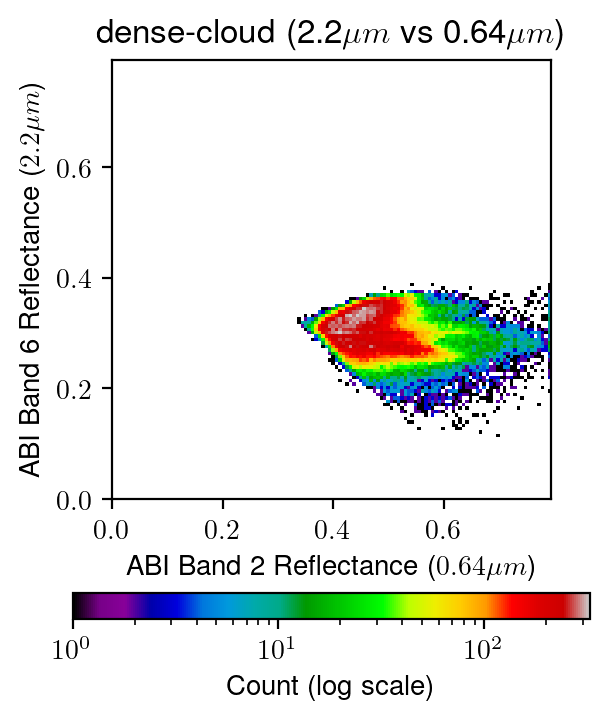
\includegraphics[width=.39\paperwidth]{figs/heatmap_b2b6_dense-cloud.png}
            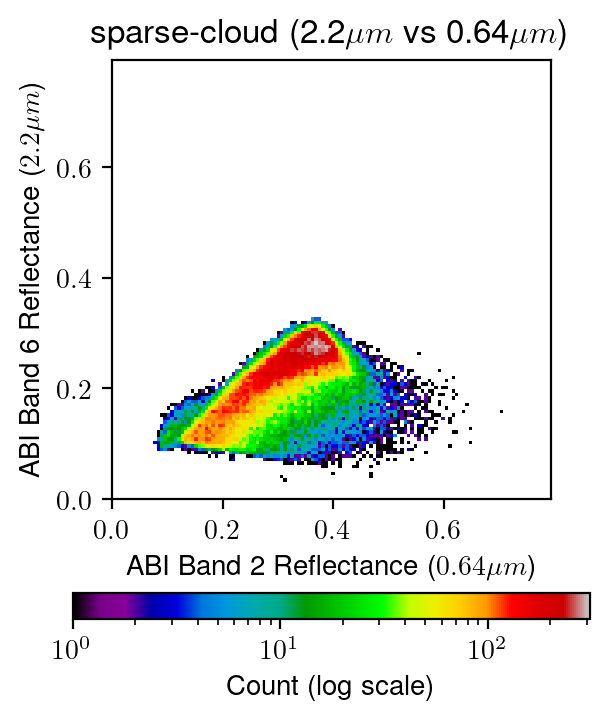
\includegraphics[width=.39\paperwidth]{figs/heatmap_b2b6_sparse-cloud.png}
        }

        \makebox[\textwidth]{
            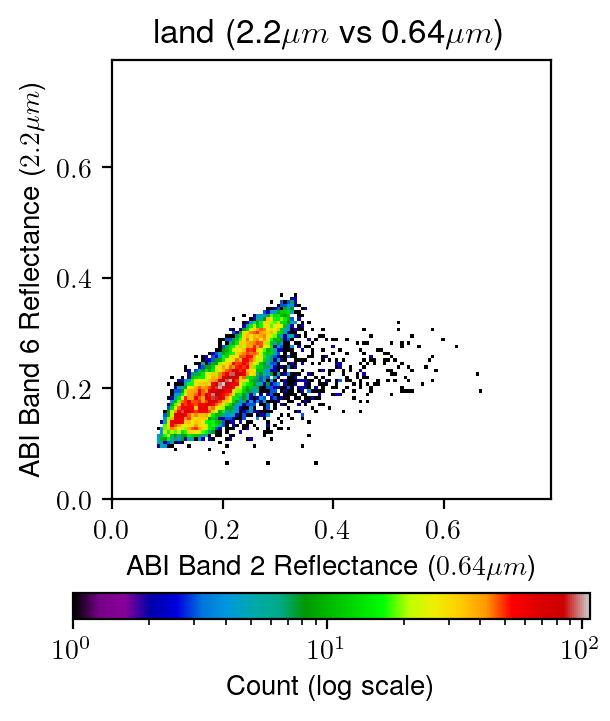
\includegraphics[width=.39\paperwidth]{figs/heatmap_b2b6_land.png}
            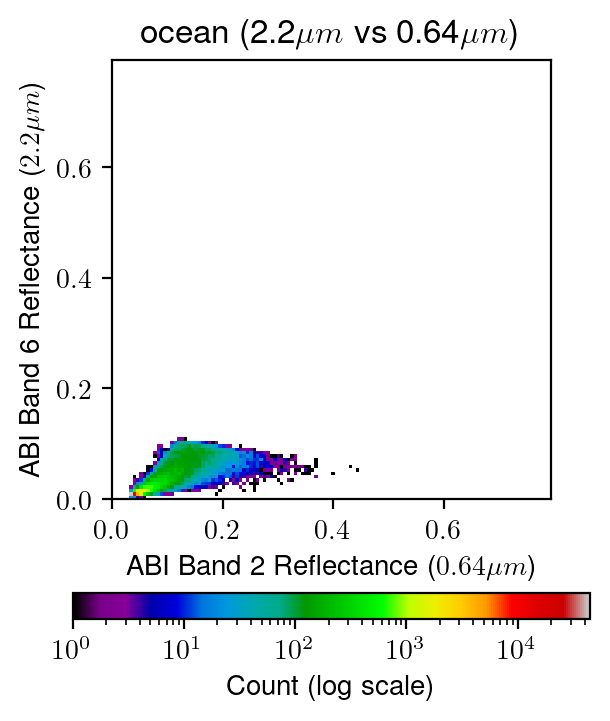
\includegraphics[width=.39\paperwidth]{figs/heatmap_b2b6_ocean.png}
        }
    \end{center}
    \caption{Bispectral diagrams of surface types in ABI Band 2 ($0.64\mu m$) and ABI Band 6 ($2.24\mu m$). Surfaces were classified using maximum-likelihood classification based on manually-selected pixel samples. Top: dense and sparse clouds; bottom: land and ocean.}
    \label{domain_rgbs}
\end{figure}

\section{Retrieval Domain}

\bibliography{main}

\end{document}
